\documentclass[12pt,a4paper]{article}

% ─── 1. PACKAGES ──────────────────────────────────────────────────────────────
\usepackage[utf8]{inputenc}
\usepackage[T1]{fontenc}
\usepackage{amsmath, amssymb}
\usepackage{geometry}
\usepackage{graphicx}
\usepackage{xcolor}
\usepackage{listings}
\usepackage{hyperref}
\usepackage{booktabs}
\usepackage{enumitem}
\usepackage{tcolorbox}
\usepackage{mdframed}
\usepackage{fancyhdr}
\usepackage{titlesec}
\usepackage{tikz} 
\usetikzlibrary{shapes.geometric, positioning, arrows.meta, calc, decorations.pathreplacing}

% Font Settings
\usepackage{newtxtext,newtxmath} % Times New Roman
\usepackage{courier}             % Courier New untuk kode

\geometry{margin=2.5cm}

% ─── 2. WARNA TEMA ────────────────────────────────────────────────────────────
\definecolor{codebg}{RGB}{245,247,250}
\definecolor{codeframe}{RGB}{180,195,215}
\definecolor{keywordcolor}{RGB}{0,112,192}
\definecolor{commentcolor}{RGB}{100,160,100}
\definecolor{stringcolor}{RGB}{180,70,50}
\definecolor{notebg}{RGB}{255,249,230}
\definecolor{noteframe}{RGB}{230,180,50}
\definecolor{tipbg}{RGB}{230,245,235}
\definecolor{tipframe}{RGB}{50,160,90}
\definecolor{sectioncolor}{RGB}{30,80,150}

% ─── 3. STYLE SECTION & TOC ───────────────────────────────────────────────────
\titleformat{\section}{\Large\bfseries\color{sectioncolor}}{}{0em}{\thesection\quad}[\titlerule]
\titleformat{\subsection}{\large\bfseries\color{sectioncolor!80}}{}{0em}{\thesubsection\quad}

% Style Table of Contents
\usepackage{tocloft}
\renewcommand{\cftsecleader}{\cftdotfill{\cftdotsep}}
\renewcommand{\cftsecfont}{\bfseries\color{sectioncolor}}

% ─── 4. LISTINGS (CODE STYLE) ─────────────────────────────────────────────────
\lstdefinestyle{customstyle}{
  basicstyle=\ttfamily\small,
  backgroundcolor=\color{codebg},
  frame=single,
  rulecolor=\color{codeframe},
  keywordstyle=\bfseries\color{keywordcolor},
  commentstyle=\itshape\color{commentcolor},
  stringstyle=\color{stringcolor},
  numbers=left,
  numberstyle=\tiny\color{gray},
  breaklines=true,
  tabsize=4,
  showstringspaces=false
}
\lstset{style=customstyle}

% ─── 5. KOTAK CATATAN (MD-FRAME) ──────────────────────────────────────────────
\newmdenv[
  backgroundcolor=notebg, linecolor=noteframe, linewidth=2pt,
  leftline=true, topline=false, rightline=false, bottomline=false,
  innerleftmargin=10pt, innertopmargin=6pt, innerbottommargin=6pt, skipabove=8pt
]{notebox}

\newmdenv[
  backgroundcolor=tipbg, linecolor=tipframe, linewidth=2pt,
  leftline=true, topline=false, rightline=false, bottomline=false,
  innerleftmargin=10pt, innertopmargin=6pt, innerbottommargin=6pt, skipabove=8pt
]{tipbox}

% ─── 6. HEADER & FOOTER ───────────────────────────────────────────────────────
\pagestyle{fancy}
\fancyhf{}
\fancyhead[L]{\small\textit{Metodologi Penelitian}}
\fancyhead[R]{\small\textit{noteify -- Statistik Deskriptif}}
\fancyfoot[C]{\thepage}
\renewcommand{\headrulewidth}{0.4pt}

% ─── 7. DATA COVER ────────────────────────────────────────────────────────────
\title{
  {\LARGE\bfseries METODOLOGI PENELITIAN}\\[0.5em]
  {\large Modul Pembelajaran: Statistik Deskriptif}\\[0.8em]
  {\normalsize Penjelasan komprehensif mengenai konsep tendensi sentral, analisis sebaran data, perhitungan varians dan simpangan baku, distribusi normal, juling data, serta aplikasi komputasinya dalam SPSS.}
}
\author{}
\date{}

% ==============================================================================
\begin{document}

\maketitle
\thispagestyle{fancy}
\tableofcontents
\newpage

% ─── KONTEN MATERI ─────────────────────────────────────────────────────────────

\section{Pengantar Statistik Deskriptif}

Sebelum peneliti melangkah jauh melakukan pengujian hipotesis (statistik inferensial), langkah esensial pertama yang wajib dilakukan terhadap sekumpulan data mentah adalah \textbf{Statistik Deskriptif}. Sesuai dengan namanya, fungsi utama dari tahap ini adalah untuk mendeskripsikan, meringkas, dan melihat gambaran besar atau "wajah asli" dari sebaran data tersebut.

Tanpa statistik deskriptif, peneliti akan buta terhadap karakteristik datanya sendiri, apakah datanya normal, apakah banyak anomali (\textit{outlier}), dan bagaimana persebarannya.

\subsection{Kecenderungan Terpusat (Central Tendency)}
Untuk mendeskripsikan suatu data, hal pertama yang dicari biasanya adalah nilai pusat atau representasi tunggal dari kelompok data tersebut. Ada tiga metrik utama yang digunakan:

\textbf{1. Rerata (Mean)} \\
Rerata aritmatika adalah rata-rata sekumpulan data. Dihitung dengan cara menjumlahkan semua nilai dan membaginya dengan banyak nilai tersebut ($\Sigma X / N$).
\begin{itemize}
    \item \textit{Contoh:} Dari skor 90, 105, 95, 100, 110, totalnya adalah 500. Reratanya adalah $500 / 5 = 100$.
    \item \textbf{Kelemahan Kritis:} Rerata \textbf{sangat dipengaruhi oleh skor ekstrim}. Sedikit saja skor yang sangat tinggi akan menarik nilai rerata naik secara drastis, dan sedikit skor yang sangat rendah akan membuat rerata anjlok.
\end{itemize}

\textbf{2. Median} \\
Median adalah bilangan tengah yang membagi daftar skor yang telah diurutkan secara numerik menjadi persis separuh atas dan separuh bawah.
\begin{itemize}
    \item Jika jumlah data ganjil: `2, 3, 5, 9, 12, 25, 37`. Mediannya adalah 9 (tiga skor di bawah, tiga di atas).
    \item Jika jumlah data genap: `2, 3, 5, 12, 25, 37`. Ambil dua skor di tengah (5 dan 12), lalu hitung reratanya $\Rightarrow (5+12)/2 = 8,5$.
    \item \textbf{Keunggulan Utama:} \textbf{Median tidak dipengaruhi oleh skor ekstrim}. Karena ia tidak terpengaruh \textit{outlier}, ia lebih baik dalam mewakili kecenderungan terpusat ketika distribusi data sedang juling (miring).
\end{itemize}

\textbf{3. Mode (Modus)} \\
Bilangan atau skor yang paling sering muncul dalam sebuah distribusi data.

\newpage
\section{Bentuk Distribusi Data}

\subsection{Distribusi Normal (Kurva Lonceng)}
Distribusi normal mendeskripsikan bagaimana data yang ideal menyebar. Ciri khasnya adalah kurva berbentuk seperti lonceng (\textit{bell-shaped}), di mana nilai pada ujung-ujung distribusi sama jaraknya ke rerata (simetris). Pada distribusi normal yang sempurna, titik puncak kurva mewakili Rerata, Median, dan Mode yang jatuh pada satu titik yang sama secara berimpit.

\subsection{Distribusi Juling (Skewness)}
Dalam kenyataannya, data sering kali memiliki nilai ekstrem (\textit{outlier}) pada salah satu ujung, yang membuat kurvanya kehilangan kesimetrisan dan menjadi juling (\textit{skew}).

\textbf{1. Juling Positif (Positively Skewed)}
\begin{itemize}
    \item Terjadi ketika terdapat sedikit nilai pada \textbf{ujung tinggi} (nilai ekstrem besar) dari rentang data.
    \item \textbf{Dampak:} Karena ada nilai super tinggi, Rerata akan ditarik menuju ujung ekstrim tersebut. Hal ini menyebabkan nilai Rerata menjadi lebih besar dan berada di sebelah kanan dari nilai Median/Mode.
\end{itemize}

\begin{figure}[h]
    \centering
    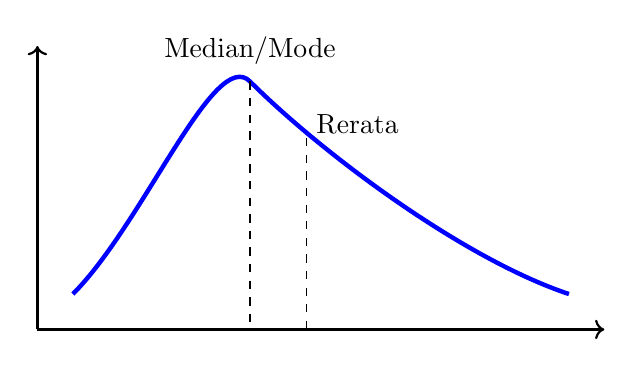
\begin{tikzpicture}[scale=0.9]
        \draw[thick, ->] (0,0) -- (8,0);
        \draw[thick, ->] (0,0) -- (0,4);
        
        \draw[blue, ultra thick] (0.5,0.5) .. controls (1.5,1.5) and (2.5,4) .. (3,3.5) .. controls (4,2.5) and (6,1) .. (7.5,0.5);
        
        \draw[dashed] (3,3.5) -- (3,0);
        \node[above] at (3,3.6) {Median/Mode \textnormal{}};
        
        \draw[dashed] (3.8,2.7) -- (3.8,0);
        \node[right] at (3.8,2.9) {Rerata \textnormal{}};
    \end{tikzpicture}
    \caption{Kurva Juling Positif. Rerata tertarik ke arah nilai ekstrem tinggi.}
\end{figure}

\textbf{2. Juling Negatif (Negatively Skewed)}
\begin{itemize}
    \item Terjadi ketika terdapat nilai pada \textbf{ujung rendah} (nilai ekstrem kecil) dari rentang data.
    \item \textbf{Dampak:} Kehadiran skor yang sangat rendah ini menyebabkan nilai Rerata turun secara drastis, menjauhi puncak kurva ke arah kiri. Akibatnya, Rerata lebih kecil daripada Median.
\end{itemize}

\begin{figure}[h]
    \centering
    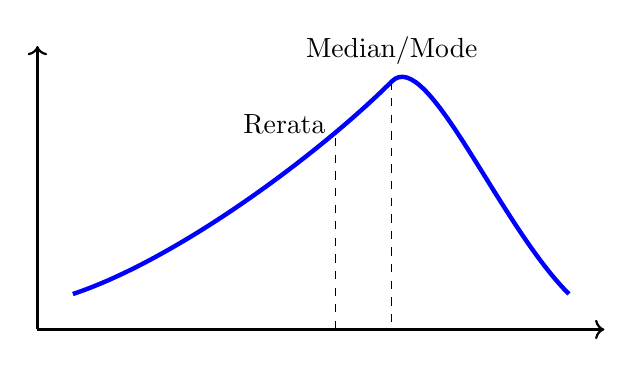
\begin{tikzpicture}[scale=0.9]
        \draw[thick, ->] (0,0) -- (8,0);
        \draw[thick, ->] (0,0) -- (0,4);
        
        \draw[blue, ultra thick] (0.5,0.5) .. controls (2,1) and (4,2.5) .. (5,3.5) .. controls (5.5,4) and (6.5,1.5) .. (7.5,0.5);
        
        \draw[dashed] (5,3.5) -- (5,0);
        \node[above] at (5,3.6) {Median/Mode \textnormal{}};
        
        \draw[dashed] (4.2,2.7) -- (4.2,0);
        \node[left] at (4.2,2.9) {Rerata \textnormal{}};
    \end{tikzpicture}
    \caption{Kurva Juling Negatif. Rerata anjlok ketarik nilai ekstrem rendah.}
\end{figure}

\newpage
\section{Penyebaran Data: Varians \& Simpangan Baku}

Mengetahui rata-rata saja tidaklah cukup. Kita harus tahu seberapa jauh data-data tersebut menyimpang atau tersebar dari rata-ratanya. Di sinilah peran \textit{Sum of Squares}, Varians, dan Simpangan Baku.

\subsection{Rumus Matematis}
Ada perbedaan pembagi ($N$ vs $n-1$) tergantung apakah kita mengukur seluruh Populasi atau sekadar Sampel:
\begin{itemize}
    \item \textbf{Untuk Populasi:}
    $$ SS = \sum x^2 - \frac{(\sum x)^2}{N} \quad \text{dimana} \quad \sigma^2 = \frac{SS}{N} $$
    \item \textbf{Untuk Sampel:}
    $$ SS = \sum x^2 - \frac{(\sum x)^2}{n} \quad \text{dimana} \quad s^2 = \frac{SS}{n-1} $$
\end{itemize}

\subsection{Contoh Perhitungan Komprehensif}
Diberikan skor tes potensi akademik dari 10 mahasiswa ($n=10$): 450, 560, 250, 630, 280, 300, 340, 435, 355, 700. Rerata (Mean) skor ini adalah 430.
\begin{enumerate}
    \item Total $\sum x = 4300$.
    \item Total $\sum x^2 = 2.064.750$.
    \item Hitung \textbf{Sum of Squares (SS)}:
    $$ SS = 2.064.750 - \frac{(4300)^2}{10} = 2.064.750 - 1.849.000 = 215.750 $$
    \item Hitung \textbf{Varians Sampel ($s^2$)}:
    $$ s^2 = \frac{215.750}{10 - 1} = \frac{215.750}{9} = 23.972,22 $$
    \item Hitung \textbf{Simpangan Baku / Standard Deviation ($SD$)}:
    $$ SD = \sqrt{23.972,22} = 154,83 $$
\end{enumerate}

\textbf{Maknanya apa?}\\
Rerata skor adalah 430. Simpangan baku menjelaskan bahwa secara umum, skor-skor mahasiswa tersebut \textbf{menyimpang} atau bertebaran sejauh $\pm 154,83$ poin dari reratanya.

\newpage
\section{Aturan Empiris pada Kurva Normal}

Jika data berdistribusi normal, simpangan baku ($\sigma$) memiliki properti luar biasa yang disebut Aturan Empiris (68-95-99.7). 

\begin{figure}[h]
    \centering
    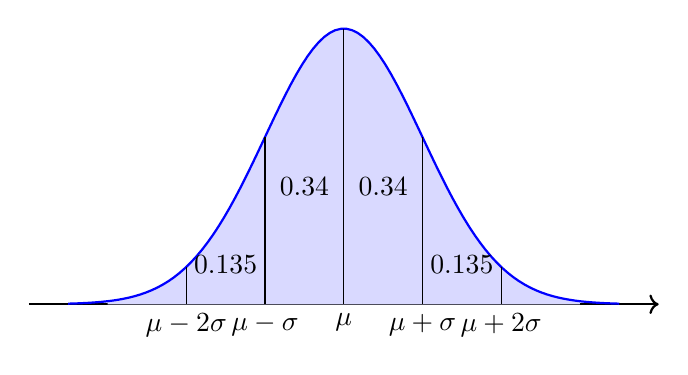
\begin{tikzpicture}[scale=1]
        % Axis
        \draw[thick, ->] (-4,0) -- (4,0);
        
        % Normal Curve
        \fill[blue!15] (-3,0) -- plot[domain=-3:3, samples=100] (\x, {3.5*exp(-0.5*\x*\x)}) -- (3,0) -- cycle;
        \draw[blue, thick] plot[domain=-3.5:3.5, samples=100] (\x, {3.5*exp(-0.5*\x*\x)});
        
        % Vertical Lines and Text for standard deviations
        \draw (-1, {3.5*exp(-0.5)}) -- (-1, 0);
        \draw (1, {3.5*exp(-0.5)}) -- (1, 0);
        \draw (-2, {3.5*exp(-2)}) -- (-2, 0);
        \draw (2, {3.5*exp(-2)}) -- (2, 0);
        \draw (0, 3.5) -- (0, 0);
        
        % Area labels
        \node at (-0.5, 1.5) {0.34 \textnormal{}};
        \node at (0.5, 1.5) {0.34 \textnormal{}};
        \node at (-1.5, 0.5) {0.135 \textnormal{}};
        \node at (1.5, 0.5) {0.135 \textnormal{}};
        
        % Axis Labels
        \node[below] at (0,0) {$\mu$};
        \node[below] at (-1,0) {$\mu-\sigma$};
        \node[below] at (1,0) {$\mu+\sigma$};
        \node[below] at (-2,0) {$\mu-2\sigma$};
        \node[below] at (2,0) {$\mu+2\sigma$};
    \end{tikzpicture}
    \caption{Luas Area Distribusi Normal Berdasarkan Simpangan Baku.}
\end{figure}

Dari kurva di atas, kita tahu bahwa persentase kasus yang jatuh di antara Rerata ($\mu$) dan $\pm 1\sigma$ adalah \textbf{34\%}. Total luas area dari $\mu - 1\sigma$ hingga $\mu + 1\sigma$ adalah $34\% + 34\% = 68\%$.

\textbf{Contoh Analisis Kasus:} \\
Diketahui sebuah distribusi memiliki Rerata = 61 dan Simpangan Baku = 7. Interval di bawah skor 68 mewakili berapa persentase skor?
\begin{itemize}
    \item Skor 68 itu setara dengan $\mu + 1\sigma$ (karena $61 + 7 = 68$).
    \item Persentase di bawah rerata 61 adalah 50\% (separuh populasi).
    \item Persentase antara 61 hingga 68 ($\mu + 1\sigma$) adalah 34\%.
    \item Jadi, $50\% + 34\% = 84\%$. Skor 68 berada pada \textbf{persentil ke-84}.
\end{itemize}

\newpage
\section{Penyajian Data \& Komputasi dengan SPSS}

Bekerja dengan data di dunia nyata hampir selalu menggunakan aplikasi perangkat lunak seperti SPSS.

\subsection{Tabel Frekuensi dan Persentase}
Tabel adalah bagian penting dari analisis data yang meringkas Frekuensi dan Persentase subjek. Contoh dari total data $N=80$:
\begin{table}[h]
\centering
\begin{tabular}{@{}lcc@{}}
\toprule
\textbf{Pekerjaan} & \textbf{Frekuensi} & \textbf{Persentase (\%)} \\ \midrule
Perawat & 17 & 21,25 \\
Guru & 3 & 3,75 \\
Presenter & 23 & 28,75 \\
Mahasiswa & 20 & 25,00 \\
Lain-lain & 17 & 21,25 \\ \bottomrule
\end{tabular}
\end{table}

\subsection{Langkah-langkah Komputasi di SPSS}
Dalam perangkat lunak SPSS, untuk mendeskripsikan data langkah umumnya adalah sebagai berikut:
\begin{enumerate}
    \item \textbf{Memasukkan Data (Input):}
    \begin{itemize}
        \item Pada menu \textit{Variable View}, buat dan beri nama variabel (misal 'Pekerjaan' atau 'Usia'). 
        \item Beri label \textit{Values} jika datanya kategori (contoh: 1 untuk 'Perawat', 2 untuk 'Guru').
        \item Masukkan angka mentahnya pada kolom di \textit{Data View}.
    \end{itemize}
    \item \textbf{Menganalisis Tendensi dan Sebaran:}
    \begin{itemize}
        \item Pilih menu \textit{Analyze $\rightarrow$ Descriptive Statistics $\rightarrow$ Frequencies...}
        \item Masukkan variabel ke kotak analisis.
        \item Klik tombol \textit{Statistics} dan centang opsi yang dibutuhkan: \textit{Mean, Median, Mode, Std Deviation, Variance}, dan \textit{Range}.
    \end{itemize}
    \item \textbf{Membuat Grafik Visual (Diagram):}
    \begin{itemize}
        \item Untuk \textbf{Diagram Pie}: Pilih \textit{Graphs $\rightarrow$ Chart Builder... $\rightarrow$ Pie/Polar}. Tarik variabel ke kotak 'Slice by?'.
        \item Untuk \textbf{Bar Chart} (Diagram Batang): Pilih \textit{Graphs $\rightarrow$ Chart Builder... $\rightarrow$ Bar}. Tarik variabel ke 'X-axis?' dan atur properti elemen untuk memunculkan persentase.
        \item Kustomisasi (Edit): Diagram yang telah dirender bisa diklik dobel untuk membuka jendela properties, di mana peneliti bisa mengubah \textit{Fill} (Warna), \textit{Border}, menghapus legenda, dan memodifikasi teks label.
    \end{itemize}
\end{enumerate}

Dengan langkah-langkah di atas, tabel keluaran (Output) akan langsung menampilkan tabel Kumulatif dan Statistik Deskriptif Numerik dengan sangat presisi.

\end{document}